
\chapter{Metodologia}

{\color{red}Este capítulo dedica-se a prover uma visão geral das etapas necessárias à conclusão deste projeto, e também
permite sua eventual reprodução no futuro.}

Para a execução deste projeto, optou-se pelo uso de componentes amplamente disponíveis no mercado a relativamente baixo
custo, bem como software disponível gratuitamente no site do fabricante.


\section{Hardware}
{\color{red} Esta seção especifica os componentes físicos envolvidos no robô desenvolvido para o projeto, descrevendo
também a função de cada um no desempenho das suas funções.}
{\color{red} Inserir aqui tabela com o custo dos componentes.}

\subsection{Fabricação e montagem}
Foi decido fabricar o chassi e demais peças usando impressão 3D, com PLA.
O projeto das peças foi realizado no AutoCAD e depois modelado em 3D com SolidWorks, após a modelagem realizada,
a geometria das peças foram convertidas em código G para um impressora 3D usando o UltiMaker Cuda, a impressora usada foi a Ender 3 S1 Pro
As figuras relacionadas ao CAD, podem ser encontradas no anexo \ref{att_fabricao_montagem_cad}, quanto a modelagem,
anexo \ref{att_fabricao_montagem_modelagem}, e impressão 3D e montagem, anexo \ref{att_fabricao_montagem_impressao}.



\subsection{Motor DC e driver}
Optou-se pelo uso de um motor DC de 6V 210rpm, com taxa de redução de 1:34. O motor já possui um encoder magnético
acoplado, com 11 PPR (\textit{Pulses Per Revolution}). 
Inicialmente foi testado o driver Ponte H L298N para ligar cada motor, suporta até 2A em operação DC \cite{datasheel_l298n},
a corrente de operação máxima do motor é de 1.1A, porém a corrente de parada é drenar 3.2A. 
O L298N também causa uma queda de tensão, a 1A pode causar uma queda de 3.2V, fazendo com que o
motor não receba a tensão necessária para operar nos valores desejados \cite{datasheel_l298n}. 
O L298N é mais recomendado para tensões entre 12V a 40V, como o motor é de 6v, acaba tendo uma queda de tensão considerável.
Com isso, um driver de para baixas tensões é recomendado, foi escolhido o DRV8833 \cite{datasheel_dvr8833}.

\begin{figure}[h]
	\centering
	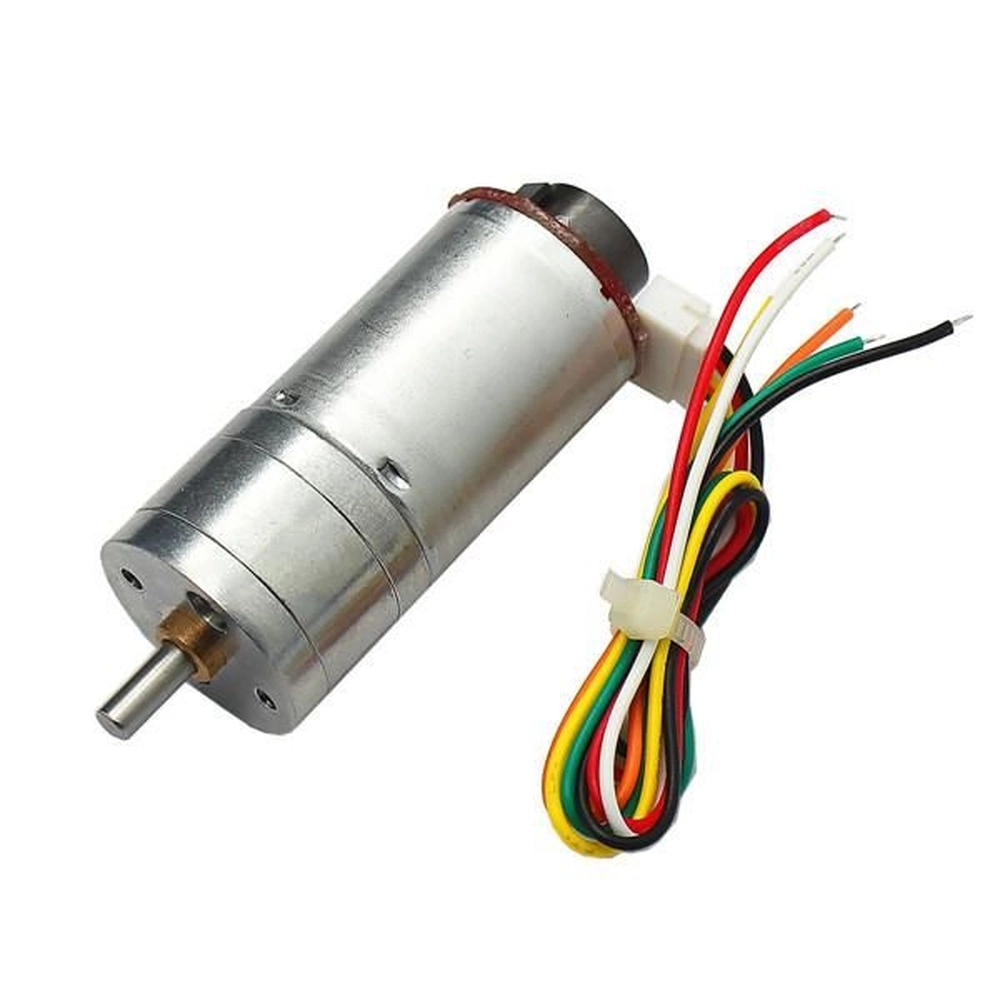
\includegraphics[width=0.7\textwidth]{figures/CHR_GM25_370}
	\caption{Motor DC 6V \cite{motor_dc_6v_encoder}}
\end{figure}


\begin{quadro}[htb]
	\caption{\label{Especificacoes_motordc_6v}Especificações do motor DC 6V}
	 \begin{tabular}{|c|c|c|c|}
		\hline
		\textbf{Componente} & \textbf{Quant} \\ \hline
		Tensão nominal & DC 6V  \\ \hline
		Velocidade sem carga  & 210RPM 0.13A  \\ \hline
		Eficiência máxima & 2,0kg.cm/170rpm/2,0W/0,60A   \\ \hline
		Poder máximo & 5,2kg.cm/110rpm/3,1W/1,10A   \\ \hline
		Torque de parada  & 10kg.cm 3.2A    \\ \hline
		Taxa de Redução do Retardador & 1:34  \\ \hline
		Resolução do salão & Razão Hall x 34,02 = 341,2PPR  \\ \hline
	\end{tabular}
	\fonte{\cite{chinhai_motor}}
	\end{quadro}

\begin{figure}[h]
	\centering
	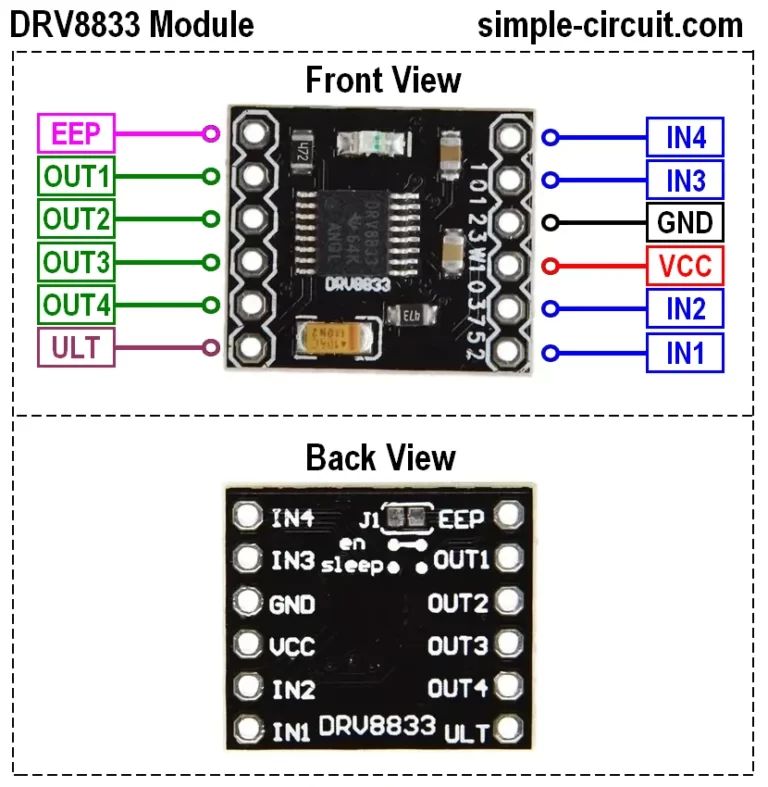
\includegraphics[width=0.7\textwidth]{figures/DRV8833-Dual-Driver-Pinout}
	\caption{Driver Ponte H DVR8833 \cite{DRV8833_image}}
\end{figure}

\subsection{Microcontrolador}

Para microcontrolador, optou-se pelo uso do  STM32F103C8, também conhecido como Blue Pill.
Possui como processador o ARM Cortex-M3, e tem 64Kbs de memória flash. 
O STM32F103C8 possui 7 timers, 2 ADCs, e 9 interfaces de comunicação, incluindo
I2C (\textit{Inter-Integrated Circuit}), USART (\textit{Universal Synchronous
Asynchronous Receiver Transmitter}), SPI (\textit{Serial Peripheral Interface}),
CAN e USB 2.0.
O STM32F103C8 possui 6 que suportam canais de PWM de 5V, e outros 8 canais de 3.3V,  e pode ser alimentado via micro
USB de 5V.

Para carregar o projeto no microcontrolador, um gravador ST-LINK USB será utilizado.

\begin{figure}[h]
	\centering
	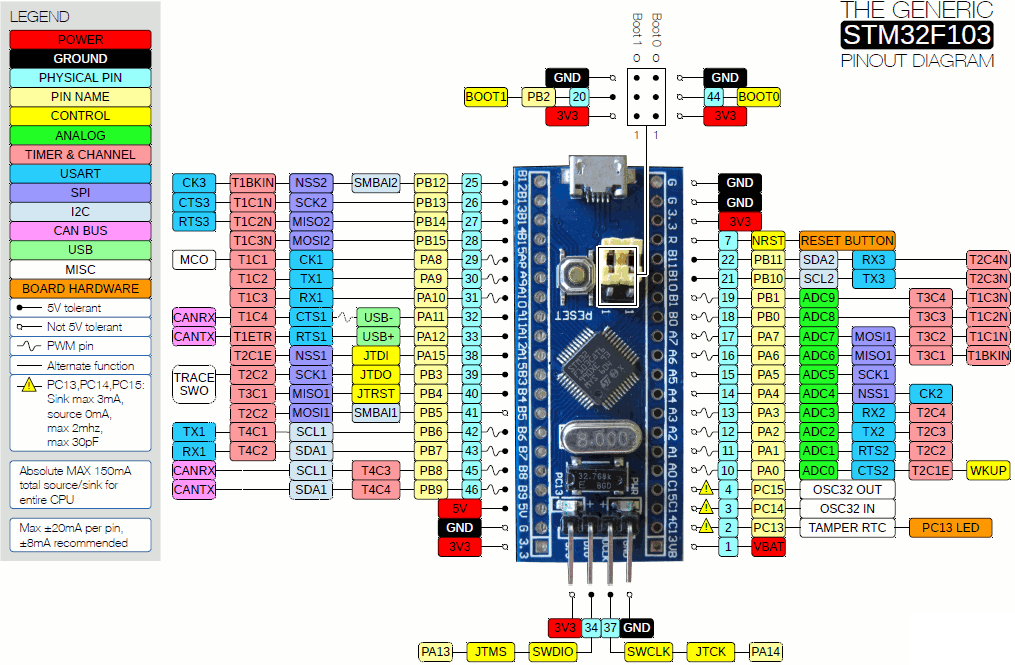
\includegraphics[width=0.8\textwidth]{figures/stm32f1_pinout}
	\caption{Diagrama de pinos do STM32F103C8}
\end{figure}

\subsection{Alimentação}
Para alimentar o microcontrolador, um powerbank com saida de 5v será usado, considerando que o STM32F103C8 funciona a
uma corrente abaixo de 100mA. Para alimentar os motores, para uso no desenvolvimento, optou-se por uma bateria de chumbo-ácido de 6V 4.5Ah

% \subsection{Joystick de controle}
% Um joystick de 3 eixos para controlar o robô para testar a cinemática de movimento.
% {\color{red} É necessário aqui especificar o modelo utilizado e descrever características.}

% \subsection{Sensores}
% {\color{red} Esta subseção deve descrever os sensores utilizados e também sua finalidade.}

% \subsection{Dispositivos de comunicação}
% {\color{red} Esta subseção deve descrever os dispositivos de comunicação utilizados (Wi-fi, Bluetooth, etc) e também sua
% finalidade.}

% \subsection{Calibração de parâmetros}
% {\color{red} Caso haja necessidade de calibração de parâmetros de alguns dos componentes utilizados (sensibilidade de
% sensores, histerese de componentes mecânicos, taxa de comunicação de dispositivos, etc), os procedimentos devem ser
% descritos nesta subseção.}

\section{Software}
{\color{red} Esta seção se dedica a discorrer a respeito dos diversos componentes de software envolvidos no projeto.}

